\section{Literature Review}

\subsection{Background}
Cloud architecture suffers often from an exaggeration of past issues while trying to leverage recent technologies at a rapid pace. In the cloud native world, the network is unreliable; thus, while developing bigger and more dispersed systems, the network needs to be taken into account from the outset of application design (\cite{posta2022Design}). Implementing network resilience like retries, timeouts, circuit breakers, observability, and security became challenging for application developers; hence, a decentralized application networking infrastructure was born as service mesh. Istio is one such open source implementation that has been used for a while now and has been battle tested by many corporations with their business critical applications. Istio specifies an architecture consisting of a control plane for proxy management and a data plane for network traffic and security management on behalf of an application using application layer proxies (\cite{posta2022Layers}). These application layer proxies sit as a sidecar attached to each service workload in a Kubernetes environment, making a tight-coupled architecture for service deployment. Istio's sidecar proxy injection provides significant advantages over microservice code refactoring for non-functional requirements but does not offer a perfect separation between applications and the Istio data plane (\cite{istioHoward2022}). Istio contributors explored the options of having less invasive and better ergonomic approaches in service mesh over the last few years, and as a result, ambient mesh was born. It is now possible to get rid of sidecar architecture in Istio by introducing a shared agent model running at the host level. This optimizes compute resource usage and gives the operator greater flexibility in adopting service mesh in their environment. Ambient mesh brings a lot of new excitement to the service mesh space without compromising any of the purposes that it was invented for.

\subsection{Service Mesh Origins}
During the early days of the Internet, applications used to ship their own TCP/IP stack. This implies that all networking layer code is either packed with the application or the language specific libraries are linked with the application binary. With the next generation of application development, people started shifting towards a shared library model, which is still the case with many desktop or embedded applications today. Then the three-tier application architecture paradigm arises to serve the vast majority of web applications, followed by the service-oriented architecture. This new architecture forced the developers to think the way they handled things previously. With this new decoupled service-oriented architecture, additional requirements related to connectivity, security, and observability have emerged. Resiliency became one of the most important things, including inter-service communication over non-trusted networks. In cloud based application development, the network is not limited to any particular premises boundaries; hence, a security advancement is required to a point where sender and recipient can mutually authenticate and establish a secure communication channel.

\begin{figure}[ht!]
  \centering
  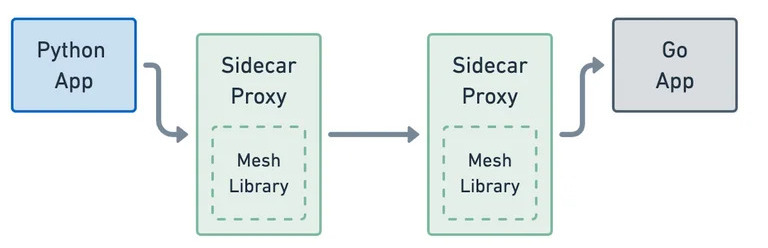
\includegraphics[width=0.7\linewidth]{resources/sidecar-design.jpg}
  \caption{Sidecar proxy design (\cite{isovalentGraf2021})}
  \label{lr:sidecarDesign}
\end{figure}

Implementing all of these functionalities in the target application or shared libraries was a big task, and making them available as part of the infrastructure for use by all applications was another big challenge. As a solution, the sidecar model is introduced, which eliminates application code modification while supporting the polyglot nature of microservice development at the same time. The term 'sidecar' is adopted as it attached to the microservices, much like a sidecar attached to a motorcycle. This sidecar is now placed with each Kubernetes workload to anticipate network or security movements inside a cluster to form a service mesh, delivering speed to the development teams to focus on business logic. Overall, service mesh is a way to connect multiple services to one consistent network and observability layer (\cite{posedioNeumer2021}).

\subsection{Shift to Kernel Model from Shared Library}
\label{lr:ebpf}
Historically, the operating system has always been an ideal place to implement observability, security, and networking functionality (\cite{ebpfIODocs}). As the operating system implements the central controller unit called the kernel, it has the unique capacity of monitoring and managing the entire system. Innovations at the kernel level have become less complex, being more complex than the functionality running outside. But with eBPF, that has changed in the last few years. What JavaScript delivered in web browsers to change the way today's web application works, eBPF is somewhat comparable technology for Linux kernel space. eBPF is a revolutionary technology that runs sand-boxed programs in the kernel without modifying the kernel source code or injecting an external kernel module to extend its functionality. Essentially, it's a runtime in the kernel, including a JIT compiler to compile byte codes into machine code for execution, making it very optimized and having a similar level of performance as native kernel code. eBPF adds the dynamic ability to program kernels by removing back-and-forth calls between kernel and user space. eBPF works at the kernel and user space levels using an event-driven hook pattern. These events include the entry or exit from any routine in kernel or user space, trace points, and most importantly, the arrival of network packets, which is crucial for any service mesh (\cite{thenewstackRice2021}). This makes eBPF extremely useful for host-level networking observability, security, and traffic management.

\begin{figure}[ht!]
  \centering
  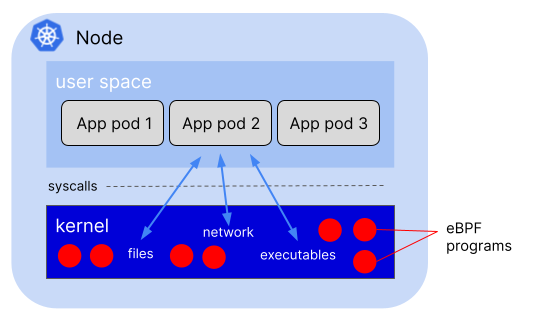
\includegraphics[width=0.65\linewidth]{resources/ebpf-service-mesh.png}
  \caption{eBPF implementation of service mesh (\cite{thenewstackRice2021})}
  \label{lr:ebpfDesign}
 \end{figure}

 As there is only one kernel per Kubernetes node, this eBPF technology has become prominent for service mesh development as it allows for only one dynamic program for the kernel to serve the service mesh functionalities. This eBPF application program acts as a proxy, but in this case, instead of attaching to each pod in the Kubernetes cluster, it is attached to the Kubernetes node. When attaching a proxy to the kernel, a one-to-one mapping is formed between the kernel and proxy, eliminating the need to inject sidecar proxies per pod. The evolution from shared libraries to sidecars and now to the kernel model for non-functional requirements in application development has really gone through a massive change, and at each stage, the significance was clearly seen by the practitioners.

\subsection{Ambient Mesh Architecture}
With the Istio 1.18.0 release in June 2023, the first open source alpha version of Ambient Mesh is launched. This new release gives an option to run Istio installation with ambient mode to forgo sidecar proxies in favor of a mesh data plane integrated into Kubernetes infrastructure (\cite{istioHoward2022}). To understand ambient mesh architecture, a quick look into the Istio sidecar architecture is required. Istio has a data plane and a control plane, where the data plane is built using the sidecar proxy injected into each Kubernetes pod. This adds functionality like monitoring, traffic routing, and policy enforcement, among many others, to and from the service to the mesh network. The control plane remains the controller unit for the data plane, and it is centrally located in the cluster. The ambient mesh divides the data plane into two segments: the secure L4 processing layer and the L7 processing layer. This layering allows the operator to use the basic potential of a service mesh by deploying only the L4 processing layer, reducing the overhead for the entire system. The layered approach also helps in migration from a no-mesh system to a secure overlay and to full L7 processing. The next two paragraphs will explore these layers along with the ambient mesh components, which form the sidecar-less architecture.

\subsubsection{L4 Secure Overlay Layer}
Layer 4 of the OSI model represents the transport layer, which provides a transparent view of data transfer between end users. Traditionally, service mesh incorporates both the L4 transport layer and the L7 application layer in a single sidecar entity, but in ambient mesh, this is separated and a new zero trust proxy, or Ztunnel, is introduced. This component is written from the ground up using one of the most efficient programming languages, Rust, which naively supports network optimizations and packet filtering. Ztunnel concentrates on a limited number of capabilities, such as \Gls{mtlsfull}, authentication, L4 authorization, and telemetry, without interrupting or processing application-level HTTP headers (\cite{istioSun2023}). Ztunnel is deployed as a daemon set on every Kubernetes node to process the basic service mesh capabilities. It also forwards the request to the intended microservice after gathering L4 metrics such as the quantity of request or response bytes. When the target microservice is running on a different node, it ensures that the data is sent to the respective Ztunnel over a secure \glsxtrshort{mtls} connection. The following diagram illustrates how Ztunnel intercepts communication for every pod that is deployed on the same node.

\begin{figure}[ht!]
  \centering
  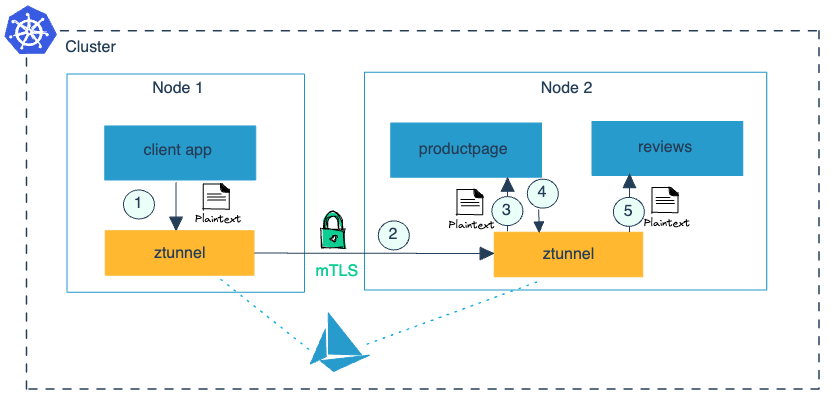
\includegraphics[width=0.7\linewidth]{resources/ambient-routing-l4.png}
  \caption{In cluster routing with Ztunnel in Ambient mesh}
  \label{lr:ztunnelDesign}
\end{figure}

\ref{lr:ztunnelDesign} depicts how a client application accepts requests from end users to serve a product page along with its reviews. The application runs on a Kubernetes cluster with two nodes, where the UI, product, and review microservice pods are spread across multiple nodes. Each node has its own Ztunnel, which internally communicates over mTLS to provide a response back to the end user.

 \subsubsection{L7 Processing Layer}
 Layer 7 works at the highest level of the OSI model where application details are available; hence, detailed HTTP-level filtering can be done. L7 processing is intensive as it intends to provide connectivity, shape the traffic, apply policies, and provide mTLS for microservices running across nodes. This intensive layer analyzes a lot of data and processes a massive scale of network traffic, utilizing more CPU and memory resources. To reduce this burden, ambient mesh introduces a shared component called Waypoint Proxy, which works per namespace or per Kubernetes service account level. Waypoint proxies can be placed on any Kubernetes node, irrespective of where the microservice pods are hosted. The Waypoint proxy forwards the request to the Ztunnel running on the same or different node as the destination microservice, but not before enforcing the L7 rules and gathering L7 metrics (\cite{glooDocs}). By default, mTLS is used to secure traffic between Ztunnel and the Waypoint proxy.

 \begin{figure}[ht!]
  \centering
  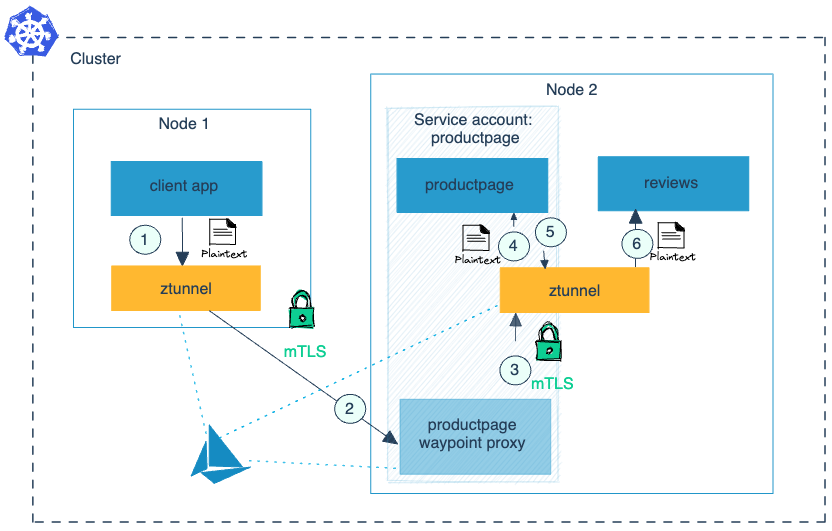
\includegraphics[width=0.7\linewidth]{resources/ambient-routing-l7.png}
  \caption{L7 routing in Ambient mesh}
  \label{lr:waypointDesign}
 \end{figure}

As shown in Figure \ref{lr:waypointDesign}, the Waypoint proxy is deployed in the product page service account. The request from the client application first reaches the Ztunnel of the client microservice node and is routed to the Waypoint proxy. This is possible as L7 traffic policies are applied to the product page. On receiving the request, the Waypoint proxy performs the L7 processing, such as collecting metrics and forwarding them to the Ztunnel of the corresponding node where the product page microservice pod is running.

\subsection{Value Proposition of Ambient Mesh}
Grey literature describes how, using the sidecar-less model, one can reduce the number of proxy instances significantly. One of the empirical studies (\cite{thenewstackRice2021}) mentions that using a service mesh built on top of eBPF technology can cut down the proxy counts from 100 to just 3 in a complex Kubernetes cluster used in production. In some other articles, the problem of sidecar proxies is discussed in a real-life scenario. \cite{mediumSinghal2021} mentions how they faced a massive increase in memory usage per proxy from 60–70 MiB to 700 MiB–1.2 GiB when they shifted from a small Kubernetes cluster to a larger one. The root cause was identified in the same article, and the solution was to restrict the proxy to the required namespaces so that it does not ingest network traffic data for all the services running in the cluster. But even with this limited proxy configuration, per-node memory utilization could reach a significant number when the service replica increases due to auto-scaling. Kernel mode service mesh not only reduces this memory footprint, but it can also reduce the complexity of having less configuration and eliminate microservice pod restarts when rolling out the service mesh in a live cluster. Though the focal point of kernel mode service meshes like ambient mesh remains on the performance side, the reduced operational complexities cannot be ignored. One of the most significant benefits of switching to ambient mesh is two layers of network traffic filtering. Ambient mesh allows incremental adoption by applying secure overlay processing by default and high-level HTTP-based L7 processing on demand. This two-layer architecture enables organizations to pay for what is needed and scale the service mesh data plane independently from the Kubernetes workload, reducing the infrastructure cost (\cite{infoqSunCampbell2023}).

\subsection{Summary}
Ambient mesh offers advantages over sidecar based deployment models due to its noninvasive and leaner design. Adoption of the ambient mesh directly reduces infrastructure costs and improves performance because it involves fewer components: Ztunnel proxies per node and the optional Waypoint proxy. The design also allows for separating L4 and L7 processing, giving the operator granularity in control and choice. Though the introduction of ambient mesh does not mean the end of the sidecar model in service mesh, there is a lot of potential that it brings today. There are use cases where service meshes with sidecars may remain useful, such as in regulatory environments where keeping proxies in the same pod guarantees that they are coupled with microservices, which is easy to justify during an audit. Despite a few exceptional cases, ambient mesh will remain one of the most exciting technologies in the service mesh and Kubernetes fields, which leverage the Linux kernel eBPF technology. As there is no academic research paper available at present, an immense opportunity is opened to explore ambient mesh, what it offers, and how it is different from the sidecar mode of Istio.